%
% File acl2019.tex
%
%% Based on the style files for ACL 2018, NAACL 2018/19, which were
%% Based on the style files for ACL-2015, with some improvements
%%  taken from the NAACL-2016 style
%% Based on the style files for ACL-2014, which were, in turn,
%% based on ACL-2013, ACL-2012, ACL-2011, ACL-2010, ACL-IJCNLP-2009,
%% EACL-2009, IJCNLP-2008...
%% Based on the style files for EACL 2006 by
%%e.agirre@ehu.es or Sergi.Balari@uab.es
%% and that of ACL 08 by Joakim Nivre and Noah Smith
% chktex-file 19
% chktex-file 13
% chktex-file 24
% chktex-file 8
% chktex-file 44
% chktex-file 45
% chktex-file 46

\documentclass[11pt,a4paper]{article}
\usepackage[hyperref]{acl2019}
\usepackage{times}
\usepackage{latexsym}
\usepackage{url}

\usepackage{listings}
\usepackage{multirow}
\lstset{basicstyle=\ttfamily, keywordstyle=\rmfamily\bfseries}

\usepackage[final]{graphicx}
\usepackage{amsmath,amssymb}
\usepackage{algorithm}
\usepackage{pgfplots}
\usepackage{enumerate}
\usepackage{url}
\usepackage[outdir=./]{epstopdf}
\usepackage{flushend}
\usepackage[most]{tcolorbox}
\setlength{\fboxsep}{2pt}
\usepackage[T1]{fontenc}
\usepackage[utf8]{inputenc}
\usepackage[russian,english]{babel}


%\aclfinalcopy % Uncomment this line for the final submission
%\def\aclpaperid{***} %  Enter the acl Paper ID here

%\setlength\titlebox{5cm}
% You can expand the titlebox if you need extra space
% to show all the authors. Please do not make the titlebox
% smaller than 5cm (the original size); we will check this
% in the camera-ready version and ask you to change it back.

\newcommand\BibTeX{B\textsc{ib}\TeX}

\title{Zero-shot WordNet Construction using Cross-lingual Embeddings}

\author{Denis Gordeev, Alexey Rey, Dmitry Shagarov
	First Author \\
  Affiliation / Address line 1 \\
  Affiliation / Address line 2 \\
  Affiliation / Address line 3 \\
  \texttt{email@domain} \\\And
  Second Author \\
  Affiliation / Address line 1 \\
  Affiliation / Address line 2 \\
  Affiliation / Address line 3 \\
  \texttt{email@domain} \\}

\date{}

\begin{document}
\maketitle
\begin{abstract}
Low-resource languages often lack structured text representations (taxonomies, ontologies and lexical databases). In this paper we propose a method for constructing WordNets without translation data or parallel corpora. The proposed method outperforms translation-based techniques in F1-score. We also publish automatedly constructed truncated WordNets for 44 languages (including non-European ones).
\end{abstract}

\section{Introduction}
%ворднеты делали
%рассказать про русские ворднеты
%упомянуть другие ворднеты
%и про ходака

There are numerous structured information representations containing texts as titles, descriptions or definitions: e.g.\ ontologies, taxonomies, and lexical databases. Among such databases we can highlight WordNet\cite{wordnet}. WordNet is a lexical database covering various types of relations between words: both semantical and lexical. Semantic concepts called synsets are connected in accordance to the semantic and lexical relations between them. It has found a very broad usage for many natural language processing and machine learning tasks \cite{kutuzovgraphwordnet,mao-semeval}.
There have been many attempts by researchers to automatically convert WordNet from English into other languages. Most attempts were focused on using machine translation engines, extensive bilingual dictionaries or parallel corpora~\cite{Khodak2017,NEALE18.1030} which are often lacking for low-resource languages.

In this paper we propose a method for constructing WordNets using cross-lingual embeddings. Unlike previous attempts our method does not require translation engines or parallel corpora. There have been already works using word embeddings for extending existing WordNets \cite{sand2017wordnet,tarouti} in monolingual settings. However, these methods could not be used for creating a WordNet for another language from scratch.

Word embeddings proved to be a powerful tool for dense text representations after papers by Bengio~\cite{bengio} and Mikolov~\cite{mikolov-representations-2013}. However, first word vector representation models were monolingual only. Soon researchers proposed cross-lingual word embedding models~\cite{mikolov-parallel}. There followed several improvements to the original model. In \citeyear{artetxe2016learning} Arxetxe et al. found that Procrustes refinement gets better results than the original linear transformation method by Mikolov. Also most earlier methods suffered from the "hubness problem" where some words (especially low frequency ones) appear in the top neighbour lists of many other words.

Alexis Conneau et al. in \citeyear{muse} offered a method called cross-domain similarity local scaling (CSLS) to overcome this problem. They have reached 81.7\% accuracy for English-Spanish and 83.7\% for Spanish-English pairs for top-1500 source queries in a completely unsupervised mode. For English-Russian and Russian-English their results are not as high and they achieved accuracy of 51.7\% and 63.7\% respectively. Their FastText embeddings were trained on Wikipedia datasets for each respective language. Also they have published aligned embeddings for 30 languages \footnote{https://github.com/facebookresearch/MUSE}. Joulin et al. in \citeyear{joulin2018loss} found that convex relaxations of the CSLS loss improves the quality of bilingual word alignment. Also they have published aligned FastText vectors with vocabularies exceeding 2 million words and phrases \footnote{https://fasttext.cc/docs/en/aligned-vectors.html}.

\section{Cross-lingual embeddings}

MUSE is based on the work by Conneau et al.~\cite{muse}. It consists of two algorithms. The first one which is used only in unsupervised cases is a pair of adversarial neural networks. The first neural network is trained to predict from which distribution $\{X, Y\}$ embeddings come. The second neural networks is trained to modify embeddings $X$ multiplying it by matrix $W$ to prevent the first neural network from making accurate discriminations. Thus, at the end of the training we get a matrix $WX$ which is aligned with matrix $Y$.

\begin{figure}
	
	\centering
	\small
	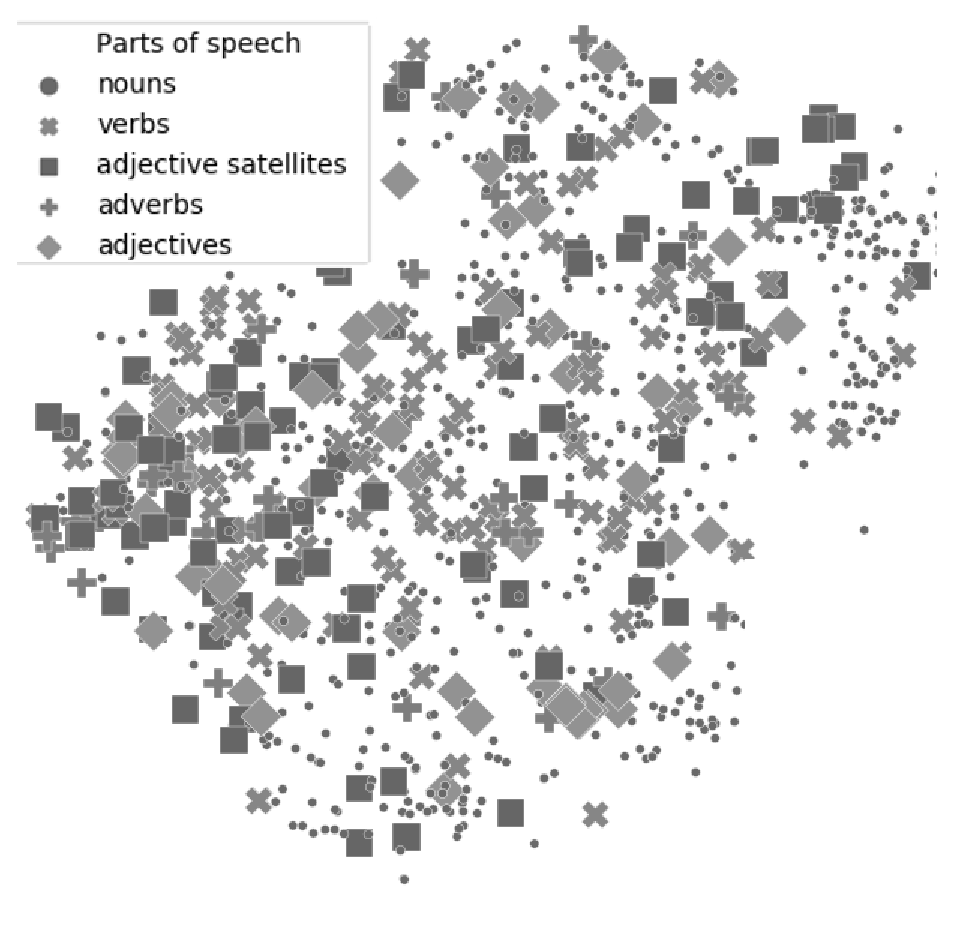
\includegraphics[scale=0.5]{wordnet-pos2}\\
	
	\caption{TSNE visualisation of WordNet synset SIF-embeddings}
	\label{wordnet-pos}
\end{figure}

The second method is supervised and the aim is to find a linear mapping $W$ between embedding spaces $X$ and $Y$ which can be solved using Orthogonal Procrustes problem:

$$ W^* = argmin_W ||WX - Y||_F = UV^T$$

where $UV^T$ is derived using singular value decomposition SVD$(YX^T) = U \Sigma V^T$
This method is used iteratively with the default number of iterations in MUSE equal to 5. As Søgaard, Ruder and Vulić state Procrustes refinement relies on frequent word pairs to serve as reliable anchors.

Conneau et al.\ also apply cross-domain similarity local scaling to lessen the extent of hubness problem which cross-lingual embeddings are prone to~\cite{dinu}. It uses cosine similarity between a source embedding vector $x$ and $k$ target nearest embeddings $\mathcal{N}$ (the default $k$ in MUSE is 10) to generate a dictionary.
\begin{align*}
sim(x, y) = \dfrac{1}{k}\sum_{i=1}^K\cos(x, {\mathcal{N}_X}_i);\\
\mathcal{N}_X \in Y=\{y_1,...,y_n\} 
\end{align*}
\small
$$CSLS(x,y) = 2\cos(x,y) - sim_{source}(x, y)  - sim_{target}(y, x)$$
\normalsize

Vecmap~\cite{vecmap} is close in its idea to the Procrustes refinement, it computes SVD-factorization SVD$(YX^T) = U\Sigma V^T$ and replaces $X$ and $Y$ with new matrices $X' = U$ and $Y' = V$. The authors also propose normalization and whitening (sphering) transformation. After applying whitening new matrices are equal to:
$X' = {({X^T}X)}^{-\tfrac{1}{2}}$ and $Y' = {({Y^T}Y)}^{-\tfrac{1}{2}}$

Jawanpuria et al.~\cite{jawanpuria} propose a method which is also based on SVD-factorization but in smooth Riemannian manifolds instead of Euclidean space.

Joulin et al. in \citeyear{joulin2018loss} introduced a reformulation of CSLS that generalizes to convex functions (Relaxed CSLS loss). Due to the orthogonality constraint on $W$ and FastText vectors being $\ell_2$-normalized $\cos(Wx, y) = x^T W^Ty$ and $|| y - {W_X}_i ||^2_2 = 2 - 2x^TW^Ty$. The problem can be reformulated to find the $k$ elements of $Y$ which have the largest dot product with ${W_X}_i$. Thus, RCSLS can be written down as:
\begin{align*}
\underset{W \in  \mathcal O_d}{min} \dfrac{1}{n}\sum_{i=1}^{n} - 2x^T_iW^Ty_i \\
+ \dfrac{1}{k} \sum_{y_j \in \mathcal{N}_Y({W_X}_i)}^{ } x_i^T W^Ty_j \\
+ \dfrac{1}{k} \sum_{{W_X}_j \in \mathcal{N}_X(y_i)}^{ } x_j^T W^Ty_i
\end{align*}
Thus, RCSLS can be solved using manifold optimization tools \cite{boumal2014manopt}.
\section{Experiments}
We reformulated the problem of synset finding as a binary classification problem. The task is to predict for the given (synset, lemma) pair if they are related or not. As the training/validation data we used English Princeton WordNet \cite{wordnet} provided by the NLTK package~\cite{nltk}. It contains 117'659 synsets. As positive examples we use (lemma, synset) pairs. As negative examples lemmas from other synsets with the same root are used (chicken.n.01 vs. chicken.n.02). We also added some random words because of the lack of negative examples. There were also attempts at augmenting the training data with the information from the Open Multilingual WordNet \cite{bond-wordnet}. We used only Finnish Open WordNet because it is 100\% full and allows to avoid bias towards Indo-European languages used for testing.

	\begin{table}[!htbp]
	\small
	\caption{Training data for chicken.n.01 (the flesh of a chicken used for food)}
	\label{wordnet-training-data}		
	\centering
	\begin{tabular}{|l|l|l|}
		\hline
		Word & Synset & Target
		\\
		\hline
		chicken & chicken.n.01 & 1
		\\
		poulet & chicken.n.01 & 1
		\\
		yellow & chicken.n.01 & 0
		\\
		chickenhearted & chicken.n.01 & 0
		\\
		visible & chicken.n.01 & 0
		\\
		\hline
	\end{tabular}
	
\end{table}

Synset embeddings were calculated using averaged synset lemma embedding and the definition embedding. We used averaging weights 0.2 for the lemma and 0.8 for the definition. SIF and TFIDF-averaging schemes were used for definition embeddings. SIF \cite{Arora2017} embeddings use pre-trained word vectors. For each sentence $s$ this model first creates a vectorized averaged representation $V_s$.

$$V_s = \dfrac{1}{|s|}\sum_{w \in s} \frac{a}{a + p(w)}V_w$$
where $V_w$ is the word unigram probability and $a$ is a scalar (set to 1e-3 by default).
After that all sentence embeddings are grouped into a matrix where $u$ is its first singular vector. The final sentence embedding is computed using this singular vector $u$.
$$V_s = V_s - uu^TV_s$$

For each lemma we used its embedding from the corresponding cross-lingual pre-trained model (\cite{muse} or \cite{joulin2018loss}) for the language.

Predicting synset relations is not a trivial task even in a monolingual setting. E.g. we failed to get any meaningful cluster representation for synsets using TSNE \cite{tsne} (Fig. \ref{wordnet-pos}). Moreover, there is not much training data and models are prone to overfitting. Thus, we introduced an ensemble of 4 LGBM-models \cite{lgbm} and 4 dense 3-layered fully-connected neural networks with dropout as regularization \cite{dropout}.
In our case fine-tuning parameters using half of data not only did not bring any benefit to the final score but even decreased it significantly.

We also attempted to fine tune input data using PCA and UMAP embeddings but it did not provide any benefit and actually decreased results.


\section{Multiword Expressions}
Mikolov bigrams
\section{WordNet construction}
WordNet construction imposes significant computational problems because for every word from the vocabulary we need to compare it with every possible synset. For this reason we used several heuristics. 1) removed strings with punctuation besides the underscore symbol. 2) identified language using <cite> for each string.
Vectorized all computations
Preselected words using a simple model with a low threshold (0.2).
\section{Results}

As can be seen from table \ref{wordnet-results}

	\begin{table*}[!htbp]
	\small
	\caption{Results for WordNet-synset prediction}
	\label{wordnet-results}		
	\centering
	\begin{tabular}{l l l l}
		Method & POS & F1 French & F1 Russian
		\\
		\hline
		\multirow{4}{*}{Extended Open Multilingual Wordnet \newline \cite{bond-wordnet}}
		& \multicolumn{1}{l}{Adj.} & \multicolumn{1}{l}{40.8} & \multicolumn{1}{l}{41.3} \\
		& \multicolumn{1}{l}{Noun} & \multicolumn{1}{l}{43.8} & \multicolumn{1}{l}{53.1} \\
		& \multicolumn{1}{l}{Verb} & \multicolumn{1}{l}{29.4} & \multicolumn{1}{l}{34.8} \\
		& \multicolumn{1}{l}{Total} & \multicolumn{1}{l}{38.0} & \multicolumn{1}{l}{43.1} \\
		\hline
		\multirow{4}{*}{Synset Representation + Linear-WSI \cite{Khodak2017}}
		& \multicolumn{1}{l}{Adj.} & \multicolumn{1}{l}{62.5} & \multicolumn{1}{l}{64.9} \\
		& \multicolumn{1}{l}{Noun} & \multicolumn{1}{l}{66.0} & \multicolumn{1}{l}{\textbf{67.61}} \\
		& \multicolumn{1}{l}{Verb} & \multicolumn{1}{l}{55.9} & \multicolumn{1}{l}{49.7} \\
		& \multicolumn{1}{l}{Total} & \multicolumn{1}{l}{61.5} & \multicolumn{1}{l}{60.7} \\
		
		\hline
		\multirow{4}{*}{Ensemble model (SIF + Non-English data + RCSLS)}
		& \multicolumn{1}{l}{Adj.} & \multicolumn{1}{l}{\textbf{62.8}} & \multicolumn{1}{l}{\textbf{65.0}} \\
		& \multicolumn{1}{l}{Noun} & \multicolumn{1}{l}{\textbf{71.8}} & \multicolumn{1}{l}{65.1} \\
		& \multicolumn{1}{l}{Verb} & \multicolumn{1}{l}{60.0} & \multicolumn{1}{l}{\textbf{54.8}} \\
		& \multicolumn{1}{l}{Total} & \multicolumn{1}{l}{\textbf{64.1}} & \multicolumn{1}{l}{\textbf{61.0}} \\
		
		\hline
		\multirow{4}{*}{Ensemble model (SIF + \textbf{Only-English} data + RCSLS)}
		& \multicolumn{1}{l}{Adj.} & \multicolumn{1}{l}{62.3} & \multicolumn{1}{l}{64.6} \\
		& \multicolumn{1}{l}{Noun} & \multicolumn{1}{l}{70.9} & \multicolumn{1}{l}{63.6} \\
		& \multicolumn{1}{l}{Verb} & \multicolumn{1}{l}{\textbf{60.3}} & \multicolumn{1}{l}{53.6} \\
		& \multicolumn{1}{l}{Total} & \multicolumn{1}{l}{63.9} & \multicolumn{1}{l}{60.1} \\
		\hline
		\multirow{4}{*}{Ensemble model (SIF + Non-English data + \textbf{MUSE})}
		& \multicolumn{1}{l}{Adj.} & \multicolumn{1}{l}{61.0} & \multicolumn{1}{l}{64.8} \\
		& \multicolumn{1}{l}{Noun} & \multicolumn{1}{l}{71.3} & \multicolumn{1}{l}{64.1} \\
		& \multicolumn{1}{l}{Verb} & \multicolumn{1}{l}{59.0} & \multicolumn{1}{l}{54.3} \\
		& \multicolumn{1}{l}{Total} & \multicolumn{1}{l}{63.9} & \multicolumn{1}{l}{60.5} \\
		\hline
		\multirow{4}{*}{Ensemble model (\textbf{TFIDF} + Non-English data + RCSLS)}
		& \multicolumn{1}{l}{Adj.} & \multicolumn{1}{l}{62.3} & \multicolumn{1}{l}{63.0} \\
		& \multicolumn{1}{l}{Noun} & \multicolumn{1}{l}{68.1} & \multicolumn{1}{l}{59.5} \\
		& \multicolumn{1}{l}{Verb} & \multicolumn{1}{l}{53.9} & \multicolumn{1}{l}{48.0} \\
		& \multicolumn{1}{l}{Total} & \multicolumn{1}{l}{60.7} & \multicolumn{1}{l}{56.5} \\
		\hline
		\multirow{4}{*}{Single \textbf{LGBM}-model (SIF + Non-English data + RCSLS)}
		& \multicolumn{1}{l}{Adj.} & \multicolumn{1}{l}{59.4} & \multicolumn{1}{l}{61.4} \\
		& \multicolumn{1}{l}{Noun} & \multicolumn{1}{l}{69.2} & \multicolumn{1}{l}{63.4} \\
		& \multicolumn{1}{l}{Verb} & \multicolumn{1}{l}{57.5} & \multicolumn{1}{l}{49.2} \\
		& \multicolumn{1}{l}{Total} & \multicolumn{1}{l}{61.3} & \multicolumn{1}{l}{57.0} \\
		
		\hline
		\multirow{4}{*}{Single \textbf{NN}-model (SIF + Non-English data + RCSLS)}
		& \multicolumn{1}{l}{Adj.} & \multicolumn{1}{l}{60.5} & \multicolumn{1}{l}{62.9} \\
		& \multicolumn{1}{l}{Noun} & \multicolumn{1}{l}{69.5} & \multicolumn{1}{l}{62.5} \\
		& \multicolumn{1}{l}{Verb} & \multicolumn{1}{l}{56.3} & \multicolumn{1}{l}{51.1} \\
		& \multicolumn{1}{l}{Total} & \multicolumn{1}{l}{61.1} & \multicolumn{1}{l}{58.5} \\
		
	\end{tabular}
	
\end{table*}
\section{Conclusion}

\section{Phraser}
Moreover, what we find amusing is that English validation set results are similar to the results for the test set in another language.

Many researchers have used a similar method for detecting new hypernyms-hyponyms relations beyond WordNet for English. The work by \cite{sanchez2017well} has provided an overview of such methods. After getting rid of noisy hypernym-hyponym samples models may achieve models may achieve up to 0.812 \% in  accuracy score.

Some works propose to change the embeddings training process to incorporate hierarchical information \cite{alsuhaibani}.

Word embeddings methods are preferable for short texts~\cite{maslova-potapov}.

\bibliographystyle{acl_natbib}
\bibliography{muse-wordnet}
\end{document}
